%==============================================================================
% File: 	MAIN.Rnw
% Author: Peter DeWitt, peter.dewitt@ucdenver.edu
% Date:
% 
% Purpose:	
%
% Change log:
% 
%==============================================================================

\documentclass[letterpaper, 10pt]{article}\usepackage[]{graphicx}\usepackage[]{color}
%% maxwidth is the original width if it is less than linewidth
%% otherwise use linewidth (to make sure the graphics do not exceed the margin)
\makeatletter
\def\maxwidth{ %
  \ifdim\Gin@nat@width>\linewidth
    \linewidth
  \else
    \Gin@nat@width
  \fi
}
\makeatother

\definecolor{fgcolor}{rgb}{0.345, 0.345, 0.345}
\newcommand{\hlnum}[1]{\textcolor[rgb]{0.686,0.059,0.569}{#1}}%
\newcommand{\hlstr}[1]{\textcolor[rgb]{0.192,0.494,0.8}{#1}}%
\newcommand{\hlcom}[1]{\textcolor[rgb]{0.678,0.584,0.686}{\textit{#1}}}%
\newcommand{\hlopt}[1]{\textcolor[rgb]{0,0,0}{#1}}%
\newcommand{\hlstd}[1]{\textcolor[rgb]{0.345,0.345,0.345}{#1}}%
\newcommand{\hlkwa}[1]{\textcolor[rgb]{0.161,0.373,0.58}{\textbf{#1}}}%
\newcommand{\hlkwb}[1]{\textcolor[rgb]{0.69,0.353,0.396}{#1}}%
\newcommand{\hlkwc}[1]{\textcolor[rgb]{0.333,0.667,0.333}{#1}}%
\newcommand{\hlkwd}[1]{\textcolor[rgb]{0.737,0.353,0.396}{\textbf{#1}}}%

\usepackage{framed}
\makeatletter
\newenvironment{kframe}{%
 \def\at@end@of@kframe{}%
 \ifinner\ifhmode%
  \def\at@end@of@kframe{\end{minipage}}%
  \begin{minipage}{\columnwidth}%
 \fi\fi%
 \def\FrameCommand##1{\hskip\@totalleftmargin \hskip-\fboxsep
 \colorbox{shadecolor}{##1}\hskip-\fboxsep
     % There is no \\@totalrightmargin, so:
     \hskip-\linewidth \hskip-\@totalleftmargin \hskip\columnwidth}%
 \MakeFramed {\advance\hsize-\width
   \@totalleftmargin\z@ \linewidth\hsize
   \@setminipage}}%
 {\par\unskip\endMakeFramed%
 \at@end@of@kframe}
\makeatother

\definecolor{shadecolor}{rgb}{.97, .97, .97}
\definecolor{messagecolor}{rgb}{0, 0, 0}
\definecolor{warningcolor}{rgb}{1, 0, 1}
\definecolor{errorcolor}{rgb}{1, 0, 0}
\newenvironment{knitrout}{}{} % an empty environment to be redefined in TeX

\usepackage{alltt}
%==============================================================================
% File: 	RCLreports2.sty
% Author: Peter DeWitt, peter.dewitt@ucdenver.edu
% Date:   March 2012
% 
% Purpose:	Preamble/style file for LaTeX reports
%
% Change log:
% 15 August 2012 - added the floatrow package options for shading in floats
% 
% 24 April 2013 - added the verbatim package and ctable package
% 
%==============================================================================

\RequirePackage{graphicx}
\RequirePackage{lastpage}
\RequirePackage{mdwlist} % used for enumerate* and itemize*
\RequirePackage[normalem]{ulem} % for sout
\RequirePackage{color, colortbl}
\RequirePackage[margin = 10pt, font=small, labelfont={bf}, justification=justified]{caption}%, format = hang]{caption}
\RequirePackage{floatrow}
\RequirePackage{xcolor}

\definecolor{mygrey}{rgb}{0.95,0.95,0.95}
\DeclareColorBox{mycolorbox}{\fcolorbox{white}{mygrey}}
\floatsetup[table]{framestyle=colorbox,colorframeset=mycolorbox,framefit=yes,heightadjust=all,framearound=all,capposition=TOP}
%\floatsetup[figure]{style=boxed,framearound=all}
\floatsetup[figure]{framestyle=colorbox,colorframeset=mycolorbox,framefit=yes,heightadjust=all,framearound=all,capposition=TOP}

\floatsetup[table]{capposition=TOP}

\RequirePackage{rotating}
\RequirePackage{array}
\RequirePackage{multirow}
\RequirePackage{longtable}
\RequirePackage{amsmath}
\RequirePackage{todonotes}
\RequirePackage{subcaption}
\RequirePackage{lscape}
\RequirePackage{multicol}
\RequirePackage{verbatim}
\RequirePackage{ctable}

%\RequirePackage{ifplatform}
%\ifwindows 
%  \RequirePackage[ansinew]{inputenc} % use when compiling on Winblows
%\else
%  \RequirePackage[utf8]{inputenc}    % use when compiling on Linux
%\fi
\RequirePackage[utf8]{inputenc}

% Use if you want to have no indent and a vertical space between paragraphs
%\setlength{\parindent}{0.0in}
%\setlength{\parskip}{0.1in}

% Hyperlinks in the pdf are wonderful, use them and make them look good too.
% Modify the link colors for the hyper links within the document
\RequirePackage{hyperref}
\definecolor{link}{rgb}{0,0,1.0}
\hypersetup{
  colorlinks, %
  citecolor = link,%
  filecolor = link,%
  linkcolor = link,%
  urlcolor  = link
}

% Headers and pagestyle
\RequirePackage{fancyhdr}

%\setlength{\textwidth}{6.25in} 
\setlength{\textwidth}{6.75in} 
\setlength{\oddsidemargin}{0.0in}
\setlength{\topmargin}{-0.25in}
\setlength{\textheight}{8.75in}

\pagestyle{fancy}
\renewcommand{\headrulewidth}{1pt}
\renewcommand{\footrulewidth}{1pt}

% Title, subtitle, author and abstract

\newcommand{\rcltitle}[1]{
  \begin{center}
    {\huge \raggedright #1 \par}
  \end{center}
}
\newcommand{\rclsubtitle}[1]{\noindent \textbf{#1} \vspace{0.1in} }

%\newcommand{\rclauthor}[2]{\noindent \textit{#1} \vspace{0.05in}
%\par \noindent \begin{minipage}{0.98\linewidth} \small #2 \end{minipage} \vspace{0.1in} }
\newcommand{\rclauthor}[2]{\noindent #1 \vspace{0.05in}
\par \noindent \begin{minipage}{0.98\linewidth} \small #2 \end{minipage} \vspace{0.1in} }
 
\newcommand{\rclabstract}[1]{
  \begin{center}
    \begin{minipage}{0.90\linewidth}
      \textbf{Abstract: } #1 
    \end{minipage}
  \end{center}}





\usepackage{paralist}

% \chead{ } 
% \cfoot{ }
% \lfoot{ }
\chead{ \bf \it DRAFT }
\lfoot{ \bf \it DRAFT }
\cfoot{ \bf \it DRAFT }

\rhead{\rightmark}
\lhead{\today} 
\rfoot{Page \thepage\space of \pageref{LastPage}}

%================================================================================
\IfFileExists{upquote.sty}{\usepackage{upquote}}{}
\begin{document}

\rcltitle{Analysis of Overall Survival and Prostate Specific Survival: An Example
data analysis report generated in R, \LaTeX, and put together via {\tt knitr}}

\rclsubtitle{Prepared for Data Analysts}

\rclauthor{Peter E. DeWitt, MS}{\par\noindent ~~University of Colorado Anschutz Medical Campus,
\par\noindent ~~Colorado School of Public Health, 
\par\noindent ~~Biostatistics and Informatics, 
\par\noindent ~~Colorado Biostatistics Consortium,
\par\noindent ~~Research Consulting Lab,
\par\noindent ~~Contact: peter.dewitt@ucdenver.edu
}

\begin{center} 
  
\includegraphics[width=0.98\textwidth]{figure/CBC}
\end{center}

\begin{center}
  \line(1,0){350}
%
%   Change Log:
%   \begin{itemize}
%     \item
%   \end{itemize}
%
% \line(1,0){350}
\end{center}

\tableofcontents
\listoftables
\listoffigures

%==============================================================================
% File: 	introduction.Rnw
% Author: Peter DeWitt, peter.dewitt@ucdenver.edu
% Date:   9 November 2013
% 
% Purpose:	introduction section to the example data analysis report
%
% Change log:
% 13 November 2013 - file created
% 
%==============================================================================

\section{Introduction \label{sec:introduction}}

An example data analysis report.  The data set is fictitious.  Consider this work
only as an example of reproducible report writing.

\paragraph{Collaboration Considerations}

This report was authored in using R, {\tt knitr}, and  \LaTeX.  While there are
many advantages to authoring reports in \LaTeX, namely reproducible research via
literate programming, there are some disadvantages as well.  If the reader would
like the plain .tex files for reference and editing please let DeWitt know and
the files will be made available.  It is expected that the collaborators for
this project will be using Microsoft Office, or similar programs, to author
manuscripts, abstracts, and posters.  The text of this .pdf report should be
easy to copy and paste into Office type products.  However, the tables in this
document may not.  

To make the process of reproducing the tables presented in this document in a
Office type software package easier html versions of the tables have been
provided to the collaborators as well.  It is important to note that there are
two files, a .css file and a .html file, which need to be in the same directory
for the rendering of the .html tables to work.  Opening the .html file in any
web browser or may be imported directly into an Office program.  These tables
will require some formatting modifications.  

Graphics presented in this report are also sent to the collaborators as
individual .pdf files.  The graphics can be provided in any major graphics
format, size, and resolution as needed.  For example, if a file is needed as a
7~inch by 7~inch .tiff file with 1200 dpi resolution, please send such requests
to DeWitt and the graphics files will be produced as needed.  Many journals have
specific requirements for graphics and provide, via the journals' websites,
guidelines for authors.

%=============%
% end of file %
%=============%


%==============================================================================
% File: 	methods.Rnw
% Author: Peter DeWitt, peter.dewitt@ucdenver.edu
% Date:
% 
% Purpose:	
%
% Change log:
% 
%==============================================================================

\section{Methods \label{sec:methods}}

Data was created and modified to be used only for example purposes.  

Data analysis was done in 
R version 3.0.2 (2013-09-25)~\cite{R-base}.  Survival analysis
was done using the {\tt survival} pacakge~\cite{R-survival} with the default
Efron method for tie handling in the Cox proportional hazard models.  Graphics
were produced via the {\tt ggplot2} package~\cite{R-ggplot2}.



%=============%
% end of file %
%=============%


%==============================================================================
% File: 	analysis.Rnw 
% Author: Peter DeWitt, peter.dewitt@ucdenver.edu 
% Date:   Nov 2013
% 
% Purpose:	analysis of the external beam radiation project : example project
% for showing the use of R, LaTeX, and knitr
%
% Change log:
% 13 Nov 2013 - file created
% 
%==============================================================================




\section{Analysis and Results \label{sec:analysis}}

\subsection{Data Set Description}
%{{{

The data contained information on the following variables and
the levels for each.  There is additional information in the data set on the
Gleason scores.  For patients with a Gleason score of 7, the primary-secondary
values of `3+4' and `4+3' are available.  The following analysis uses a Gleason Score
variable with the total score used in all cases save GS 7 which is reported with
primary-secondary delineations.  Table~\ref{tab:data_summary} on
page~\pageref{tab:data_summary} report the observed data set overall and by
Gleason score.  There is a total of 
19,039
data records avaiable for analysis.





%}}}

\subsection{Seven Year Survival}
%{{{

Table~\ref{tab:gleason_km_surv_est} reports the Kaplan-Meier estimates for
survival at 88 months, the maximum follow up time observed, for each Gleason score.  
The estimated survival by primary-secondary patterns for 
Gleason scores 7 is also reported.  







%}}}

\subsection{Primary-Secondary Levels or Sums?}
%{{{
In this section of the analysis we investigate if there is any difference in the
OS or PCSS between the primary-secondary levels by Gleason score.
Results of six separate Cox PH regression models, one to compare the
relative difference in the hazard for OS and PCSS between the two levels of
delineation in each Gleason 7, 8, or 9 score,  are reported in
Table~\ref{tab:Gleason_primary_secondary_univar}.    These results indicate
there is no statistically significant differences in the hazards between the
different delineations for Gleason 8 and 9 for either OS or PCSS.  There is a
statistically significant difference in the hazard between GS 7 (4+3) and GS 7
(3+4).

Figure~\ref{fig:OS_PCSS_GS} are the Kaplan-Meier survival curves for overall and
prostate cancer survival for each Gleason score.
Figure~\ref{fig:primary_secondary_km} show the Kaplan-Meier plots for the
primary/secondary patterns within Gleason 7, 8, and 9.  Table~\ref{tab:n_evnets}
report the number of patients at risk overall and the number of deaths observed
for each Gleason score.




\begin{figure}
  \begin{subfigure}[t]{0.48\textwidth} 
\begin{knitrout}
\definecolor{shadecolor}{rgb}{0.969, 0.969, 0.969}\color{fgcolor}

{\centering 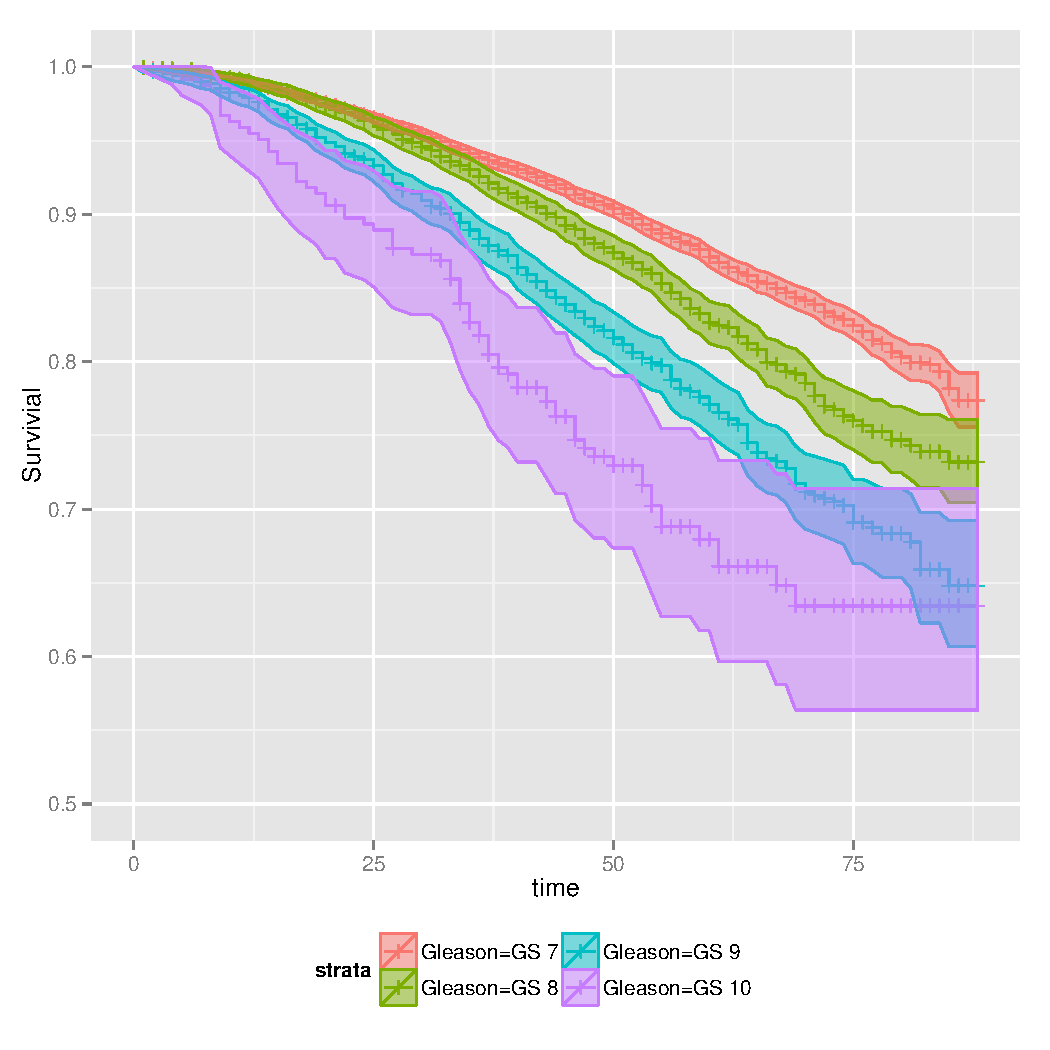
\includegraphics[width=\maxwidth]{figure/OS_GS} 

}



\end{knitrout}

    \caption{(OS\_GS.pdf) KM plot for OS by Gleason Score.}
    \label{fig:OS_GS}
  \end{subfigure}
  ~
  \begin{subfigure}[t]{0.48\textwidth} 
\begin{knitrout}
\definecolor{shadecolor}{rgb}{0.969, 0.969, 0.969}\color{fgcolor}

{\centering 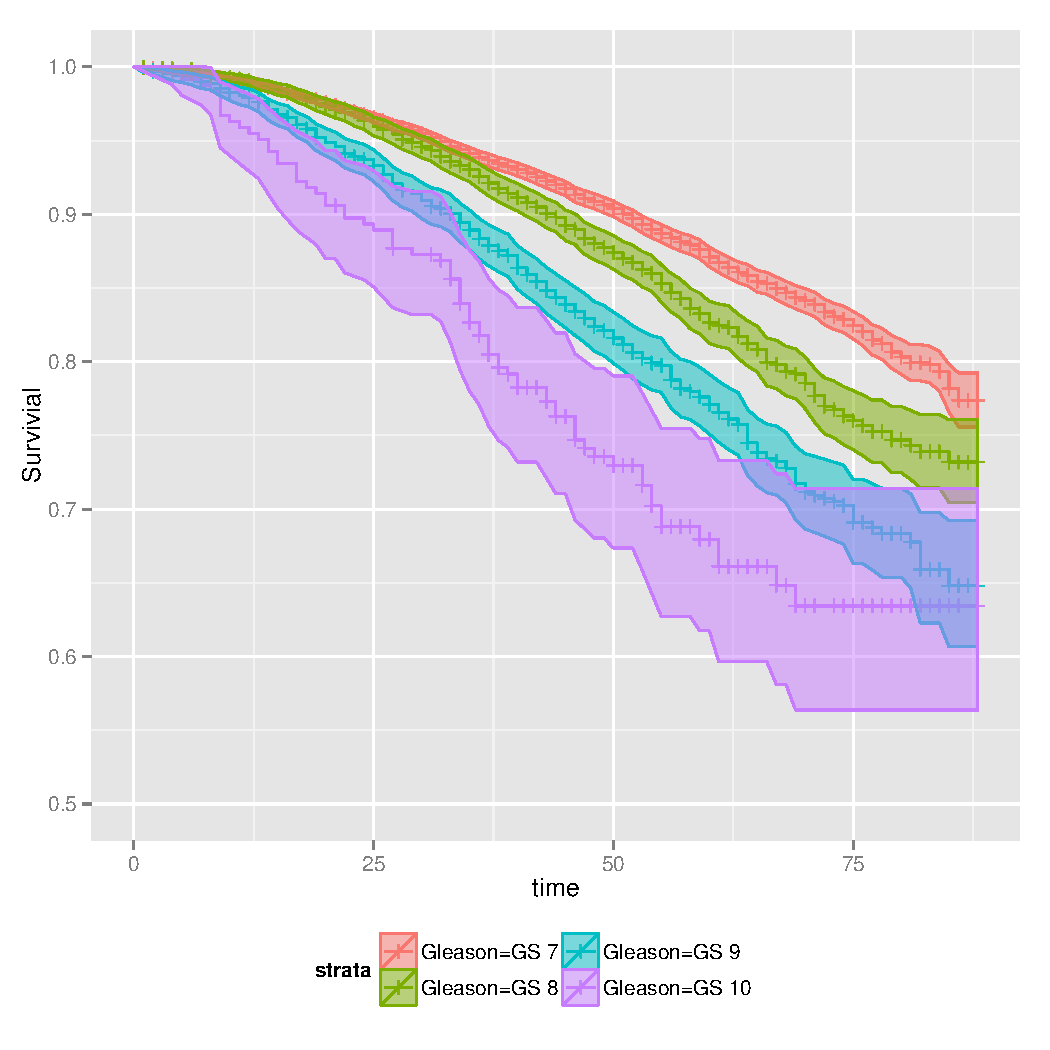
\includegraphics[width=\maxwidth]{figure/PCSS_GS} 

}



\end{knitrout}

    \caption{(PCSS\_GS.pdf) KM plot for PCSS by Gleason Score.}
    \label{fig:PCSS_GS}
  \end{subfigure}
  \caption{KM plots for OS and PCSS by Gleason Score.}
  \label{fig:OS_PCSS_GS}
\end{figure}

% KM plots
%{{{




\begin{figure}
  \begin{subfigure}[t]{0.48\textwidth}
\begin{knitrout}
\definecolor{shadecolor}{rgb}{0.969, 0.969, 0.969}\color{fgcolor}

{\centering 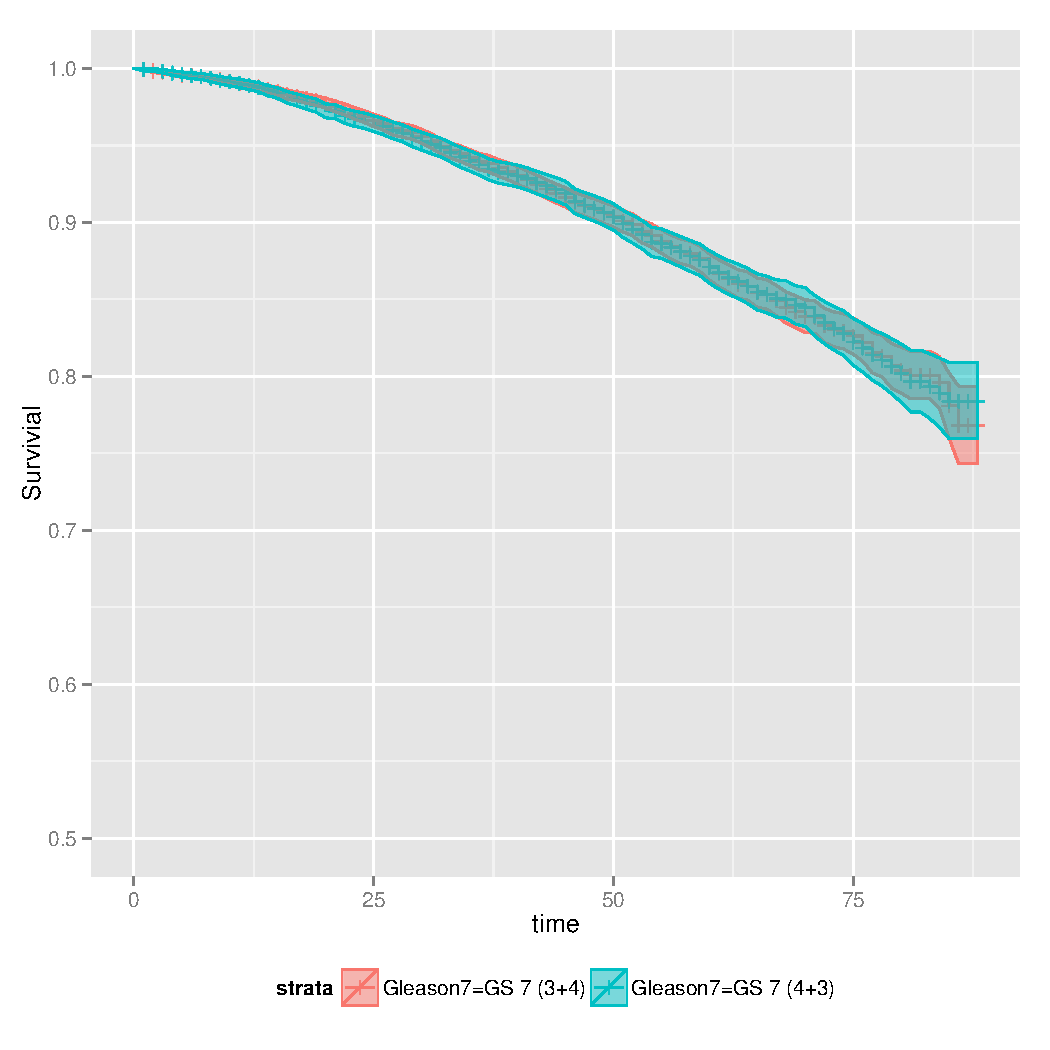
\includegraphics[width=\maxwidth]{figure/OS_Gleason7} 

}



\end{knitrout}

    \caption{(OS\_Gleason7.pdf) KM plot for OS by primary-secondary patterns
    within the 12,986 patients with a
    Gleason score of 7.}
    \label{fig:primary_secondary_km_7os}
  \end{subfigure}
  ~ 
  \begin{subfigure}[t]{0.48\textwidth}
\begin{knitrout}
\definecolor{shadecolor}{rgb}{0.969, 0.969, 0.969}\color{fgcolor}

{\centering 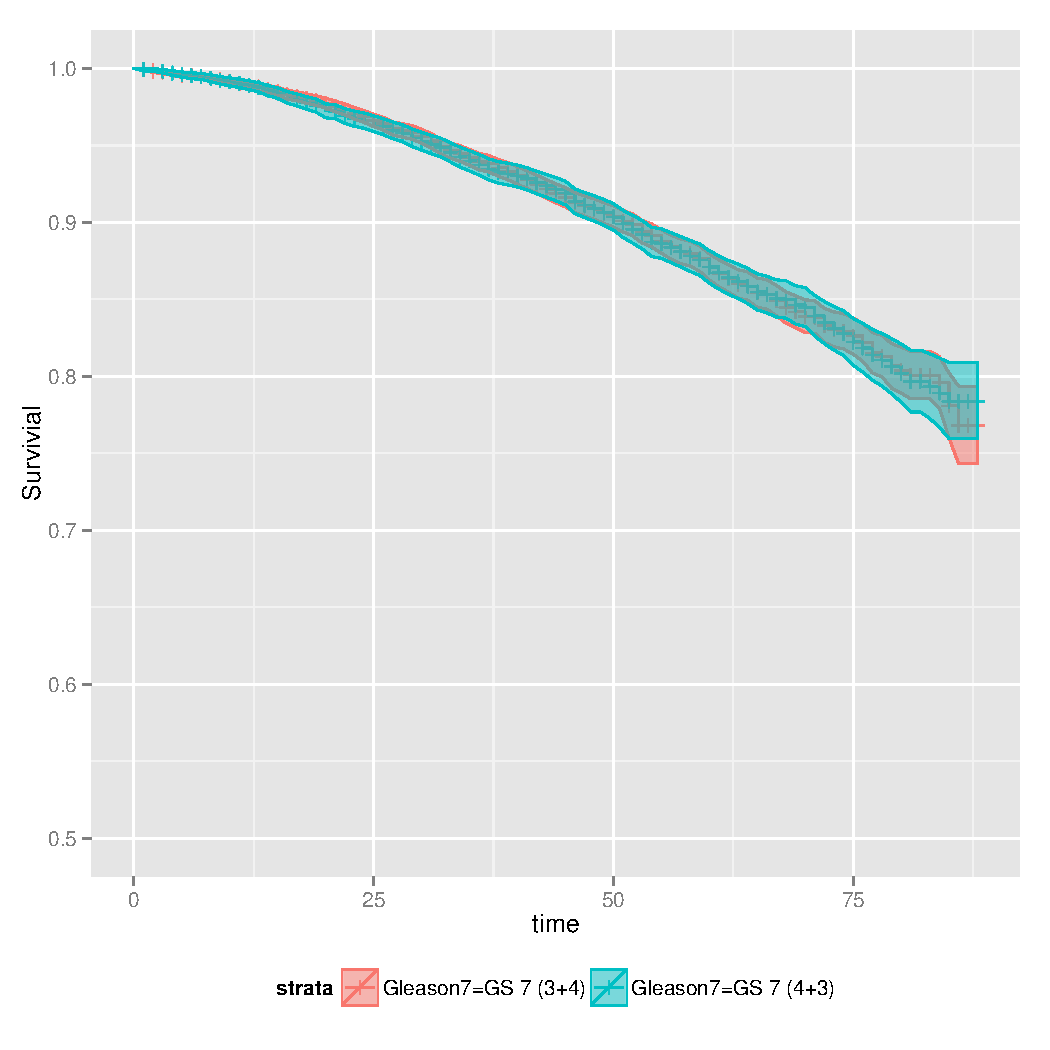
\includegraphics[width=\maxwidth]{figure/PCSS_Gleason7} 

}



\end{knitrout}

    \caption{(PCSS\_Gleason7.pdf) KM plot for PCSS by primary-secondary patterns
    within the
    12,986 patients with a Gleason score
    of 7.}
    \label{fig:primary_secondary_km_7pcss}
  \end{subfigure}
  \caption{KM plots for OS and PCSS by primary-secondary patterns for Gleason 7,
  See Table~\ref{tab:Gleason_primary_secondary_univar} for
  the log-rank test p-values.}
  \label{fig:primary_secondary_km}
\end{figure}
%}}}




%}}}

\subsubsection{Should the primary/secondary patterns be used in a multivariable
model?}  
%{{{










% in the appendix now
% % latex.default(temp, file = "../tex/os_pcss_coxph.tex", title = "",      ctable = TRUE, size = "tiny", caption = "Hazard ratios (HR) along with 95\\% confidence\n              intervals (LCL, UCL) and p-values for testing if the hazard ratio\n              is statistically different from 1 are presented in this table for\n              both univariable and multivariable regression models of both\n              overall survival and prostate cancer specific survival.",      label = "tab:os_pcss_coxph", cgroup = c("OS (univar)", "OS (multivar)",          "PCSS (univar)", "PCSS (multivar)"), n.crgoup = rep(4,          4), colhead = rep(c("HR", "LCL", "UCL", "p-value"), 4),      rgroup = rgrp, n.rgroup = nrgrp, rowname = rwnm, col.just = rep("r",          ncol(temp))) 
%
{\tiny\ctable[caption={Hazard ratios (HR) along with 95\% confidence
              intervals (LCL, UCL) and p-values for testing if the hazard ratio
              is statistically different from 1 are presented in this table for
              both univariable and multivariable regression models of both
              overall survival and prostate cancer specific survival.},label=tab:os_pcss_coxph,pos=!tbp,]{lrrrrcrrrrcrrrrcrrrr}{}{\FL
\multicolumn{1}{l}{\bfseries }&\multicolumn{4}{c}{\bfseries OS (univar)}&\multicolumn{1}{c}{\bfseries }&\multicolumn{4}{c}{\bfseries OS (multivar)}&\multicolumn{1}{c}{\bfseries }&\multicolumn{4}{c}{\bfseries PCSS (univar)}&\multicolumn{1}{c}{\bfseries }&\multicolumn{4}{c}{\bfseries PCSS (multivar)}\NN
\cline{2-5} \cline{7-10} \cline{12-15} \cline{17-20}
\multicolumn{1}{l}{}&\multicolumn{1}{c}{HR}&\multicolumn{1}{c}{LCL}&\multicolumn{1}{c}{UCL}&\multicolumn{1}{c}{p-value}&\multicolumn{1}{c}{}&\multicolumn{1}{c}{HR}&\multicolumn{1}{c}{LCL}&\multicolumn{1}{c}{UCL}&\multicolumn{1}{c}{p-value}&\multicolumn{1}{c}{}&\multicolumn{1}{c}{HR}&\multicolumn{1}{c}{LCL}&\multicolumn{1}{c}{UCL}&\multicolumn{1}{c}{p-value}&\multicolumn{1}{c}{}&\multicolumn{1}{c}{HR}&\multicolumn{1}{c}{LCL}&\multicolumn{1}{c}{UCL}&\multicolumn{1}{c}{p-value}\ML
{\bfseries Era}&&&&&&&&&&&&&&&&&&&\NN
~~Era 1&Reference&&&&&Reference&&&&&Reference&&&&&Reference&&&\NN
~~Era 2&0.83&0.76&0.90&\textless 0.001&&0.84&0.77&0.92&\textless 0.001&&0.83&0.76&0.90&\textless 0.001&&0.84&0.77&0.92&\textless 0.001\ML
{\bfseries Age}&&&&&&&&&&&&&&&&&&&\NN
~~[40,50)&Reference&&&&&Reference&&&&&Reference&&&&&Reference&&&\NN
~~[50,70)&0.95&0.84&1.09&0.481&&0.96&0.84&1.10&0.554&&0.95&0.84&1.09&0.481&&0.96&0.84&1.10&0.554\NN
~~[70,85]&1.62&1.44&1.81&\textless 0.001&&1.61&1.43&1.80&\textless 0.001&&1.62&1.44&1.81&\textless 0.001&&1.61&1.43&1.80&\textless 0.001\ML
{\bfseries T.Stage}&&&&&&&&&&&&&&&&&&&\NN
~~T Stage 1&Reference&&&&&Reference&&&&&Reference&&&&&Reference&&&\NN
~~T Stage 2&1.19&1.10&1.29&\textless 0.001&&1.12&1.03&1.21&0.006&&1.19&1.10&1.29&\textless 0.001&&1.12&1.03&1.21&0.006\NN
~~T Stage 3/4&1.54&1.34&1.77&\textless 0.001&&1.24&1.07&1.43&0.003&&1.54&1.34&1.77&\textless 0.001&&1.24&1.07&1.43&0.003\ML
{\bfseries PSA}&&&&&&&&&&&&&&&&&&&\NN
~~[0, 10) ng/ml&Reference&&&&&Reference&&&&&Reference&&&&&Reference&&&\NN
~~[10, 20) ng/ml&1.45&1.32&1.58&\textless 0.001&&1.36&1.24&1.49&\textless 0.001&&1.45&1.32&1.58&\textless 0.001&&1.36&1.24&1.49&\textless 0.001\NN
~~[20, Inf) ng/ml&1.62&1.47&1.78&\textless 0.001&&1.50&1.36&1.66&\textless 0.001&&1.62&1.47&1.78&\textless 0.001&&1.50&1.36&1.66&\textless 0.001\ML
{\bfseries Gleason7}&&&&&&&&&&&&&&&&&&&\NN
~~GS 7 (3+4)&Reference&&&&&Reference&&&&&Reference&&&&&Reference&&&\NN
~~GS 7 (4+3)&1.00&0.90&1.11&0.998&&0.99&0.90&1.10&0.915&&1.00&0.90&1.11&0.998&&0.99&0.90&1.10&0.915\NN
~~GS 8&1.34&1.21&1.48&\textless 0.001&&1.23&1.11&1.36&\textless 0.001&&1.34&1.21&1.48&\textless 0.001&&1.23&1.11&1.36&\textless 0.001\NN
~~GS 9&1.92&1.72&2.14&\textless 0.001&&1.72&1.54&1.92&\textless 0.001&&1.92&1.72&2.14&\textless 0.001&&1.72&1.54&1.92&\textless 0.001\NN
~~GS 10&2.74&2.16&3.47&\textless 0.001&&2.47&1.95&3.14&\textless 0.001&&2.74&2.16&3.47&\textless 0.001&&2.47&1.95&3.14&\textless 0.001\LL
}}


The results of the Cox proportional hazard regression models for overall
survival and prostate cancer specific survival are presented in
Table~\ref{tab:os_pcss_coxph} on page~\pageref{tab:os_pcss_coxph}.  Both
univariable and multivariable regression models are presented.  The univariable
models are built with only the noted predictor variable whereas the
multivariable models use the era, age, PSA, T Stage, and Gleason score jointly
as predictors for survival.




For overall survival we find that the patients diagnosed in Era 2
have better outcomes, i.e., longer survival, than those diagnosed
in the earlier Era 1.  For example, the hazard ratio between Era 2 and Era 1 for
overall survival based on the multivariable cox regression model is
0.84 (95\% CI: 0.77, 0.92; p \textless 0.001).

No statistically signficant difference in overall surverival was observed
between Gleason 7 (4+3) and Gleason 7 (3+4), HR = 0.99 (95\% CI: 0.90, 1.10; p = 0.915).  

Testing for a difference in the hazard ratio between sequential Gleason scores
is reported in Table~\ref{tab:sequential_hr}.  Considering that the data is
fictitious and the methods for deliniating 3+4 and 4+3 was a coin flip, it's not
surprsing that the hazard ratio between these two levels is not statistically
different from 1.  In general, and as expected for prostate cancer patients, as
the Gleason score increases the hazard increases as well.





%}}}





%=============%
% end of file %
%=============%


%==============================================================================
% File: 	conclusions.Rnw
% Author: Peter DeWitt, peter.dewitt@ucdenver.edu
% Date:
% 
% Purpose:	
%
% Change log:
% 
%==============================================================================

\section{Conclusions \label{sec:conclusions}}

Reproducible research is a growing area of concern.  Many tools exist for
literate programming and the example here is only one approach.  

Things to consider: 
\begin{itemize}
  \item portability,
  \item collaborations,
  \item robustness.
\end{itemize}

%=============%
% end of file %
%=============%



%================================================================================
% Bibliography
%




\nopagebreak[4]
\bibliographystyle{unsrt}
\bibliography{references/sources,references/R-sources}

\appendix
\begin{landscape}
  { \footnotesize % latex.default(tab1[["tab.frmt"]], file = file, title = title,      ctable = ctable, cgroup = if (missing(cgroup)) tab1[["cgrp"]] else cgroup,      n.cgroup = if (missing(n.cgroup)) tab1[["ncgrp"]] else n.cgroup,      rgroup = if (missing(rgroup)) tab1[["rgrp"]] else rgroup,      n.rgroup = if (missing(n.rgroup)) tab1[["nrgrp"]] else n.rgroup,      rowname = if (missing(rowname)) tab1[["rwnm"]] else rowname,      col.just = if (missing(col.just)) rep("r", ncol(tab1[["tab.frmt"]])) else col.just,      ...) 
%
\ctable[caption={Observed data overall and by Gleason Score.  Reported
              values are counts and row percentages, i.e., the sum of the
              reported percentages over each row should sum to 100\%.},label=tab:data_summary,pos=!tbp,]{lrrcrrcrrcrrcrrcrrcr}{}{\FL
\multicolumn{1}{l}{\bfseries }&\multicolumn{2}{c}{\bfseries Overall}&\multicolumn{1}{c}{\bfseries }&\multicolumn{2}{c}{\bfseries GS 7 (3+4)}&\multicolumn{1}{c}{\bfseries }&\multicolumn{2}{c}{\bfseries GS 7 (4+3)}&\multicolumn{1}{c}{\bfseries }&\multicolumn{2}{c}{\bfseries GS 8}&\multicolumn{1}{c}{\bfseries }&\multicolumn{2}{c}{\bfseries GS 9}&\multicolumn{1}{c}{\bfseries }&\multicolumn{2}{c}{\bfseries GS 10}&\multicolumn{1}{c}{\bfseries }&\multicolumn{1}{c}{\bfseries p-value}\NN
\cline{2-3} \cline{5-6} \cline{8-9} \cline{11-12} \cline{14-15} \cline{17-18} \cline{20-20}
\multicolumn{1}{l}{}&\multicolumn{1}{c}{n}&\multicolumn{1}{c}{\%}&\multicolumn{1}{c}{}&\multicolumn{1}{c}{n}&\multicolumn{1}{c}{\%}&\multicolumn{1}{c}{}&\multicolumn{1}{c}{n}&\multicolumn{1}{c}{\%}&\multicolumn{1}{c}{}&\multicolumn{1}{c}{n}&\multicolumn{1}{c}{\%}&\multicolumn{1}{c}{}&\multicolumn{1}{c}{n}&\multicolumn{1}{c}{\%}&\multicolumn{1}{c}{}&\multicolumn{1}{c}{n}&\multicolumn{1}{c}{\%}&\multicolumn{1}{c}{}&\multicolumn{1}{c}{}\NN
&\multicolumn{1}{c}{{\scriptsize 19,039}}&\multicolumn{1}{c}{{\scriptsize 100}}&&\multicolumn{1}{c}{{\scriptsize 7,905}}&\multicolumn{1}{c}{{\scriptsize 41.5}}&&\multicolumn{1}{c}{{\scriptsize 5,081}}&\multicolumn{1}{c}{{\scriptsize 26.7}}&&\multicolumn{1}{c}{{\scriptsize 3,670}}&\multicolumn{1}{c}{{\scriptsize 19.3}}&&\multicolumn{1}{c}{{\scriptsize 2,139}}&\multicolumn{1}{c}{{\scriptsize 11.2}}&&\multicolumn{1}{c}{{\scriptsize 244}}&\multicolumn{1}{c}{{\scriptsize 1.3}}&&\ML
{\bfseries Era}&&&&&&&&&&&&&&&&&&&\NN
~~Era 1&8,615&45.2&&3,572&41.5&&2,297&26.7&&1,659&19.3&&970&11.3&&117&1.4&&0.945\NN
~~Era 2&10,424&54.8&&4,333&41.6&&2,784&26.7&&2,011&19.3&&1,169&11.2&&127&1.2&&\ML
{\bfseries Age}&&&&&&&&&&&&&&&&&&&\NN
~~[40,50)&3,051&16.0&&1,284&42.1&&861&28.2&&544&17.8&&323&10.6&&39&1.3&&\textless 0.001\NN
~~[50,70)&5,945&31.2&&2,601&43.8&&1,658&27.9&&1,005&16.9&&608&10.2&&73&1.2&&\NN
~~[70,85]&10,043&52.7&&4,020&40.0&&2,562&25.5&&2,121&21.1&&1,208&12.0&&132&1.3&&\ML
{\bfseries T Stage}&&&&&&&&&&&&&&&&&&&\NN
~~T Stage 1&9,668&50.8&&4,334&44.8&&2,776&28.7&&1,699&17.6&&770&8.0&&89&0.9&&\textless 0.001\NN
~~T Stage 2&8,189&43.0&&3,257&39.8&&2,103&25.7&&1,657&20.2&&1,065&13.0&&107&1.3&&\NN
~~T Stage 3/4&1,182&6.2&&314&26.6&&202&17.1&&314&26.6&&304&25.7&&48&4.1&&\ML
{\bfseries PSA}&&&&&&&&&&&&&&&&&&&\NN
~~[0, 10) ng/ml&11,567&60.8&&5,148&44.5&&3,262&28.2&&1,997&17.3&&1,038&9.0&&122&1.1&&\textless 0.001\NN
~~[10, 20) ng/ml&4,372&23.0&&1,709&39.1&&1,136&26.0&&927&21.2&&531&12.1&&69&1.6&&\NN
~~[20, Inf) ng/ml&3,100&16.3&&1,048&33.8&&683&22.0&&746&24.1&&570&18.4&&53&1.7&&\LL
}
 }
\end{landscape}

% latex.default(seven.year.km, file = "../tex/gleason_km_surv_est.tex",      title = "", ctable = TRUE, caption = "Kaplan-Meier estimated survival at seven years by\n              Gleason Score.  Reported values are the estimated survival and the\n              95\\% confidence intervals for the estimated survival.",      label = "tab:gleason_km_surv_est", cgroup = c("OS", "PCSS"),      n.cgroup = c(3, 3), col.just = rep("r", ncol(seven.year.km))) 
%
\ctable[caption={Kaplan-Meier estimated survival at seven years by
              Gleason Score.  Reported values are the estimated survival and the
              95\% confidence intervals for the estimated survival.},label=tab:gleason_km_surv_est,pos=!tbp,]{lrrrcrrr}{}{\FL
\multicolumn{1}{l}{\bfseries }&\multicolumn{3}{c}{\bfseries OS}&\multicolumn{1}{c}{\bfseries }&\multicolumn{3}{c}{\bfseries PCSS}\NN
\cline{2-4} \cline{6-8}
\multicolumn{1}{l}{}&\multicolumn{1}{c}{survival}&\multicolumn{1}{c}{lower}&\multicolumn{1}{c}{upper}&\multicolumn{1}{c}{}&\multicolumn{1}{c}{survival}&\multicolumn{1}{c}{lower}&\multicolumn{1}{c}{upper}\ML
Whole Sample&76.9\%&75.8\%&78.0\%&&76.9\%&75.8\%&78.0\%\NN
Gleason 7&79.8\%&78.6\%&81.1\%&&79.8\%&78.6\%&81.1\%\NN
Gleason 7 (3+4)&80.1\%&78.5\%&81.6\%&&80.1\%&78.5\%&81.6\%\NN
Gleason 7 (4+3)&79.3\%&77.3\%&81.5\%&&79.3\%&77.3\%&81.5\%\NN
Gleason 8&73.9\%&71.4\%&76.4\%&&73.9\%&71.4\%&76.4\%\NN
Gleason 9&65.9\%&62.3\%&69.8\%&&65.9\%&62.3\%&69.8\%\NN
Gleason 10&63.4\%&56.4\%&71.4\%&&63.4\%&56.4\%&71.4\%\LL
}

% latex.default(out, file = "../tex/Gleason_primary_secondary_univar.tex",      title = "", ctable = TRUE, caption = cap, label = "tab:Gleason_primary_secondary_univar",      cgroup = c("OS", "PCSS"), n.cgroup = c(4, 4), colhead = rep(c("HR",          "LCL", "UCL", "p-value"), 2), col.just = rep("r", ncol(out))) 
%
\ctable[caption={Hazard ratios for the different primary-secondary delineations of
             the Gleason Score 7.  Results in this table are from 
             Cox Proportional Hazard models.  Reported
             results are the hazard ratios (HR), lower and upper confidence
             bounds for  95 \%
             confidence intervals and p-values are the result from log-rank
             tests for the models.},label=tab:Gleason_primary_secondary_univar,pos=!tbp,]{lrrrrcrrrr}{}{\FL
\multicolumn{1}{l}{\bfseries }&\multicolumn{4}{c}{\bfseries OS}&\multicolumn{1}{c}{\bfseries }&\multicolumn{4}{c}{\bfseries PCSS}\NN
\cline{2-5} \cline{7-10}
\multicolumn{1}{l}{}&\multicolumn{1}{c}{HR}&\multicolumn{1}{c}{LCL}&\multicolumn{1}{c}{UCL}&\multicolumn{1}{c}{p-value}&\multicolumn{1}{c}{}&\multicolumn{1}{c}{HR}&\multicolumn{1}{c}{LCL}&\multicolumn{1}{c}{UCL}&\multicolumn{1}{c}{p-value}\ML
GS 7 (3+4)&Reference&&&&&&&&\NN
GS 7 (4+3)&1.00&0.91&1.11&0.996&&1.00&0.91&1.11&0.996\LL
}

% latex.default(frmt(tab, digits = 0), file = "../tex/n_events.tex",      title = "", caption = "Number of records and number of events for OS and PCSS\n              by Gleason score and primary/secondary patterns.",      label = "tab:n_evnets", ctable = TRUE, cgroup = c("OS", "PCSS"),      n.cgroup = c(2, 2), rowgroup = gsub("Gleason=", "", rownames(tab)),      col.just = rep("r", ncol(tab))) 
%
\ctable[caption={Number of records and number of events for OS and PCSS
              by Gleason score and primary/secondary patterns.},label=tab:n_evnets,pos=!tbp,]{lrrcrr}{}{\FL
\multicolumn{1}{l}{\bfseries }&\multicolumn{2}{c}{\bfseries OS}&\multicolumn{1}{c}{\bfseries }&\multicolumn{2}{c}{\bfseries PCSS}\NN
\cline{2-3} \cline{5-6}
\multicolumn{1}{l}{}&\multicolumn{1}{c}{records}&\multicolumn{1}{c}{events}&\multicolumn{1}{c}{}&\multicolumn{1}{c}{records}&\multicolumn{1}{c}{events}\ML
Gleason=GS 7&12,986&1,611&&12,986&1,611\NN
Gleason7=GS 7 (3+4)&7,905&980&&7,905&980\NN
Gleason7=GS 7 (4+3)&5,081&631&&5,081&631\NN
Gleason=GS 8&3,670&598&&3,670&598\NN
Gleason=GS 9&2,139&473&&2,139&473\NN
Gleason=GS 10&244&73&&244&73\LL
}

% latex.default(tab, file = "../tex/sequential_hr.tex", title = "",      ctable = TRUE, caption = "Hazard ratios for sequential pairs of Gleason scores.\n              The confidence intervals and p-values have been adjusted for\n              multiple comparisons via a Bonferroni correction. These results\n              use the coefficient estimates from the multivariable Cox PH\n              regression models.",      label = "tab:sequential_hr", cgroup = c("OS", "PCSS"), n.cgroup = c(4,          4), colhead = rep(c("HR", "LCL", "UCL", "pvalue"), 2),      rgroup = rep("", 4), n.rgroup = rep(2, 4), col.just = rep("r",          ncol(tab))) 
%
\ctable[caption={Hazard ratios for sequential pairs of Gleason scores.
              The confidence intervals and p-values have been adjusted for
              multiple comparisons via a Bonferroni correction. These results
              use the coefficient estimates from the multivariable Cox PH
              regression models.},label=tab:sequential_hr,pos=!tbp,]{lrrrrcrrrr}{}{\FL
\multicolumn{1}{l}{\bfseries }&\multicolumn{4}{c}{\bfseries OS}&\multicolumn{1}{c}{\bfseries }&\multicolumn{4}{c}{\bfseries PCSS}\NN
\cline{2-5} \cline{7-10}
\multicolumn{1}{l}{}&\multicolumn{1}{c}{HR}&\multicolumn{1}{c}{LCL}&\multicolumn{1}{c}{UCL}&\multicolumn{1}{c}{pvalue}&\multicolumn{1}{c}{}&\multicolumn{1}{c}{HR}&\multicolumn{1}{c}{LCL}&\multicolumn{1}{c}{UCL}&\multicolumn{1}{c}{pvalue}\ML
{\bfseries }&&&&&&&&&\NN
~~Gleason 7 (3+4)&Reference&&&&&Reference&&&\NN
~~Gleason 7 (4+3)&0.99&0.86&1.16&1.000&&0.99&0.86&1.16&1.000\ML
{\bfseries }&&&&&&&&&\NN
~~Gleason 7 (4+3)&Reference&&&&&Reference&&&\NN
~~Gleason 8&1.23&1.04&1.46&0.001&&1.23&1.04&1.46&0.001\ML
{\bfseries }&&&&&&&&&\NN
~~Gleason 8&Reference&&&&&Reference&&&\NN
~~Gleason 9&1.40&1.17&1.68&\textless 0.001&&1.40&1.17&1.68&\textless 0.001\ML
{\bfseries }&&&&&&&&&\NN
~~Gleason 9&Reference&&&&&Reference&&&\NN
~~Gleason 10&1.44&0.99&2.08&0.016&&1.44&0.99&2.08&0.016\LL
}


\begin{landscape}
  % latex.default(temp, file = "../tex/os_pcss_coxph.tex", title = "",      ctable = TRUE, size = "tiny", caption = "Hazard ratios (HR) along with 95\\% confidence\n              intervals (LCL, UCL) and p-values for testing if the hazard ratio\n              is statistically different from 1 are presented in this table for\n              both univariable and multivariable regression models of both\n              overall survival and prostate cancer specific survival.",      label = "tab:os_pcss_coxph", cgroup = c("OS (univar)", "OS (multivar)",          "PCSS (univar)", "PCSS (multivar)"), n.crgoup = rep(4,          4), colhead = rep(c("HR", "LCL", "UCL", "p-value"), 4),      rgroup = rgrp, n.rgroup = nrgrp, rowname = rwnm, col.just = rep("r",          ncol(temp))) 
%
{\tiny\ctable[caption={Hazard ratios (HR) along with 95\% confidence
              intervals (LCL, UCL) and p-values for testing if the hazard ratio
              is statistically different from 1 are presented in this table for
              both univariable and multivariable regression models of both
              overall survival and prostate cancer specific survival.},label=tab:os_pcss_coxph,pos=!tbp,]{lrrrrcrrrrcrrrrcrrrr}{}{\FL
\multicolumn{1}{l}{\bfseries }&\multicolumn{4}{c}{\bfseries OS (univar)}&\multicolumn{1}{c}{\bfseries }&\multicolumn{4}{c}{\bfseries OS (multivar)}&\multicolumn{1}{c}{\bfseries }&\multicolumn{4}{c}{\bfseries PCSS (univar)}&\multicolumn{1}{c}{\bfseries }&\multicolumn{4}{c}{\bfseries PCSS (multivar)}\NN
\cline{2-5} \cline{7-10} \cline{12-15} \cline{17-20}
\multicolumn{1}{l}{}&\multicolumn{1}{c}{HR}&\multicolumn{1}{c}{LCL}&\multicolumn{1}{c}{UCL}&\multicolumn{1}{c}{p-value}&\multicolumn{1}{c}{}&\multicolumn{1}{c}{HR}&\multicolumn{1}{c}{LCL}&\multicolumn{1}{c}{UCL}&\multicolumn{1}{c}{p-value}&\multicolumn{1}{c}{}&\multicolumn{1}{c}{HR}&\multicolumn{1}{c}{LCL}&\multicolumn{1}{c}{UCL}&\multicolumn{1}{c}{p-value}&\multicolumn{1}{c}{}&\multicolumn{1}{c}{HR}&\multicolumn{1}{c}{LCL}&\multicolumn{1}{c}{UCL}&\multicolumn{1}{c}{p-value}\ML
{\bfseries Era}&&&&&&&&&&&&&&&&&&&\NN
~~Era 1&Reference&&&&&Reference&&&&&Reference&&&&&Reference&&&\NN
~~Era 2&0.83&0.76&0.90&\textless 0.001&&0.84&0.77&0.92&\textless 0.001&&0.83&0.76&0.90&\textless 0.001&&0.84&0.77&0.92&\textless 0.001\ML
{\bfseries Age}&&&&&&&&&&&&&&&&&&&\NN
~~[40,50)&Reference&&&&&Reference&&&&&Reference&&&&&Reference&&&\NN
~~[50,70)&0.95&0.84&1.09&0.481&&0.96&0.84&1.10&0.554&&0.95&0.84&1.09&0.481&&0.96&0.84&1.10&0.554\NN
~~[70,85]&1.62&1.44&1.81&\textless 0.001&&1.61&1.43&1.80&\textless 0.001&&1.62&1.44&1.81&\textless 0.001&&1.61&1.43&1.80&\textless 0.001\ML
{\bfseries T.Stage}&&&&&&&&&&&&&&&&&&&\NN
~~T Stage 1&Reference&&&&&Reference&&&&&Reference&&&&&Reference&&&\NN
~~T Stage 2&1.19&1.10&1.29&\textless 0.001&&1.12&1.03&1.21&0.006&&1.19&1.10&1.29&\textless 0.001&&1.12&1.03&1.21&0.006\NN
~~T Stage 3/4&1.54&1.34&1.77&\textless 0.001&&1.24&1.07&1.43&0.003&&1.54&1.34&1.77&\textless 0.001&&1.24&1.07&1.43&0.003\ML
{\bfseries PSA}&&&&&&&&&&&&&&&&&&&\NN
~~[0, 10) ng/ml&Reference&&&&&Reference&&&&&Reference&&&&&Reference&&&\NN
~~[10, 20) ng/ml&1.45&1.32&1.58&\textless 0.001&&1.36&1.24&1.49&\textless 0.001&&1.45&1.32&1.58&\textless 0.001&&1.36&1.24&1.49&\textless 0.001\NN
~~[20, Inf) ng/ml&1.62&1.47&1.78&\textless 0.001&&1.50&1.36&1.66&\textless 0.001&&1.62&1.47&1.78&\textless 0.001&&1.50&1.36&1.66&\textless 0.001\ML
{\bfseries Gleason7}&&&&&&&&&&&&&&&&&&&\NN
~~GS 7 (3+4)&Reference&&&&&Reference&&&&&Reference&&&&&Reference&&&\NN
~~GS 7 (4+3)&1.00&0.90&1.11&0.998&&0.99&0.90&1.10&0.915&&1.00&0.90&1.11&0.998&&0.99&0.90&1.10&0.915\NN
~~GS 8&1.34&1.21&1.48&\textless 0.001&&1.23&1.11&1.36&\textless 0.001&&1.34&1.21&1.48&\textless 0.001&&1.23&1.11&1.36&\textless 0.001\NN
~~GS 9&1.92&1.72&2.14&\textless 0.001&&1.72&1.54&1.92&\textless 0.001&&1.92&1.72&2.14&\textless 0.001&&1.72&1.54&1.92&\textless 0.001\NN
~~GS 10&2.74&2.16&3.47&\textless 0.001&&2.47&1.95&3.14&\textless 0.001&&2.74&2.16&3.47&\textless 0.001&&2.47&1.95&3.14&\textless 0.001\LL
}}

\end{landscape}

\end{document}         

%=============%
% end of file %
%=============%

